\documentclass[10pt,french]{book}

\input preambule_2013


\entete{\seconde 7}{Tableau de signes}{A}
\RegleEntete
\pieddepage{}{}{}

\newcommand\presentation{
\setcounter{exo}{0}
    \begin{tabular}{ll}
        Nom : \\[5pt]
        Prénom :
    \end{tabular}
\hfill
    \textbf{Note :}
        \renewcommand\arraystretch{2.3}
    \begin{tabular}{|c|}
        \hline
            \slashbox{\Huge\bfseries\phantom{10}}{\Huge\bfseries 10}\\
        \hline
    \end{tabular}
        \renewcommand\arraystretch{1.5}\par\vspace*{1cm}
    \hrulefill
}


\begin{document}


%-------------
% SUJET A
%-------------

\presentation

\exo 
\begin{enumerate}
    \item Résoudre les équations suivantes : \quad $2x - 3 = 0$ \qetq $-5x + 1 = 0$.\vspace*{5cm}
    \item Compléter le tableau de signes suivant :
    \begin{center}
        \begin{tikzpicture}
            \tkzTabInit[nocadre,espcl=2,lgt=3.5]{$x$/0.75,Signe de \\ $2x - 3$/1.5,Signe de \\ $-5x+1$/1.5,Signe de \\ $(2x - 3)(-5x+1)$/1.5}{$-\infty$,,,$+\infty$}
            \tkzTabLine{,,t,,t,}
            \tkzTabLine{,,t,,t,}
            \tkzTabLine{,,t,,t,}
        \end{tikzpicture}
    \end{center}
    \item Résoudre $(2x - 3)(-5x + 1) < 0$.\vspace*{2cm}
\end{enumerate}\[*\]

\exo
\begin{enumerate}
    \item Dresser le tableau de signes de l'expression $\dfrac{2x + 5}{-x - 4}$.
    \item Résoudre l'inéquation $\dfrac{2x + 5}{-x - 4} \leqslant 0$
\end{enumerate}

\clearpage

%-------------
% SUJET B
%-------------

\entete{\seconde 7}{Tableau de signes}{B}
\setcounter{exo}{0}

\presentation

\exo
\begin{enumerate}
    \item Résoudre les équations suivantes : \quad $-2x - 3 = 0$ \qetq $5x + 1 = 0$.\vspace*{5cm}
    \item Compléter le tableau de signes suivant :
    \begin{center}
        \begin{tikzpicture}
            \tkzTabInit[nocadre,espcl=2,lgt=3.5]{$x$/0.75,Signe de \\ $-2x - 3$/1.5,Signe de \\ $5x+1$/1.5,Signe de \\ $(-2x - 3)(5x+1)$/1.5}{$-\infty$,,,$+\infty$}
            \tkzTabLine{,,t,,t,}
            \tkzTabLine{,,t,,t,}
            \tkzTabLine{,,t,,t,}
        \end{tikzpicture}
    \end{center}
    \item Résoudre $(-2x - 3)(5x + 1) < 0$.\vspace*{2cm}
\end{enumerate}\[*\]

\exo
\begin{enumerate}
    \item Dresser le tableau de signes de l'expression $\dfrac{-2x + 5}{-x + 4}$.
    \item Résoudre l'inéquation $\dfrac{-2x + 5}{-x + 4} \geqslant 0$
\end{enumerate}

\end{document}
